The Degree Planner UI layer consists of Web application, Course catalog, Semester catalog, and Export subsystem. The main functionality of this layer is to provide the user interface, where the user is able to prepare his/her degree plan and view the related information. Among the above-mentioned subsystems, the Web application handles the most of the task, while the rest support

\subsection{Web Application}
Web application subsystem provides the user interface for the process of planning degree. The two fundamental goal of this layer is to display information and to interact with user.

\begin{figure}[h!]
	\centering
 	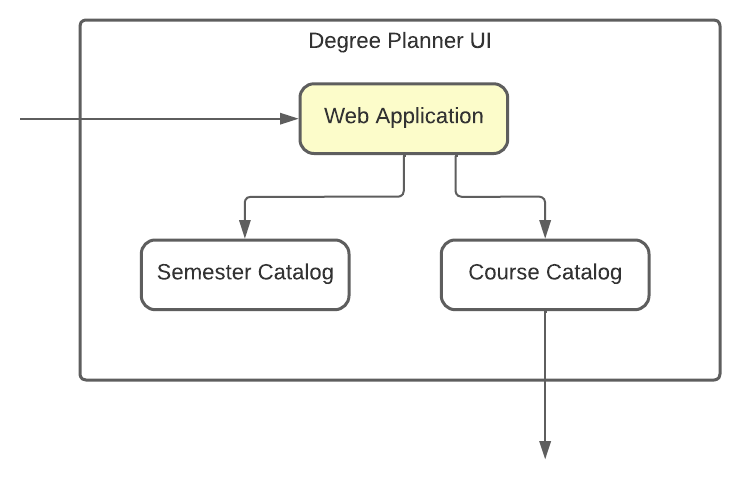
\includegraphics[width=0.60\textwidth]{images/WebApplication}
 \caption{Web Application subsystem}
\end{figure}

\subsubsection{Assumptions}
\begin{itemize}
\begin{item}
The user must have Internet connection to use the service.
\end{item}
\begin{item}
The subsystem is only available for users authenticated in Dashboard layer.
\end{item}
\begin{item}
The subsystem does not provide any functionality to modify data and no data changes should be made in this subsystem.
\end{item}
\end{itemize}

\subsubsection{Responsibilities}
This subsystem takes responsibility to display the required information, including: the user's major, list of courses for the corresponding major, list of semesters, estimated graduation date, total hours per semester, and etc. All data fetched from external sources are assumed to be up-to-date and cannot be modified in this layer. The user will perform planning tasks, such as drag and drop to add and/or remove courses. That is, the list of course objects from Course catalog subsystem will be made draggable, while the area/column for each available semester will become droppable. Besides, there will be navigation options to link to Export subsystem.

\subsubsection{Subsystem Interfaces}

\begin {table}[H]
\caption {Web Application subsystem interfaces} 
\begin{center}
    \begin{tabular}{ | p{1cm} | p{2cm} | p{6cm} | p{3cm} |}
    \hline
    ID & Description & Inputs & Outputs \\ \hline
    \#1 & Choose major & \pbox{6cm}{Option} & \pbox{3cm}{Screen}  \\ \hline
    \#2 & Display courses & \pbox{6cm}{Object of every element in the list of courses provided by Course catalog subsystem} & \pbox{3cm}{Screen}  \\ \hline
    \#3 & Search for courses & \pbox{6cm}{Text \\ Numbers} & \pbox{3cm}{Object of the searched course}  \\ \hline
    \#4 & Display semesters & \pbox{6cm}{List of semesters} & \pbox{3cm}{Screen}  \\ \hline
    \#5 & Export & \pbox{6cm}{N/A} & \pbox{3cm}{Navigation to Export subsystem}  \\ \hline
    \end{tabular}
\end{center}
\end{table}

\subsection{Course Catalog}
Course catalog subsystem acts as the interface between the Degree Planner UI layer and Firebase database layer. It will fetch data, i.e., the list of courses, from the database, and sends it to the Web application subsystem.

\begin{figure}[h!]
	\centering
 	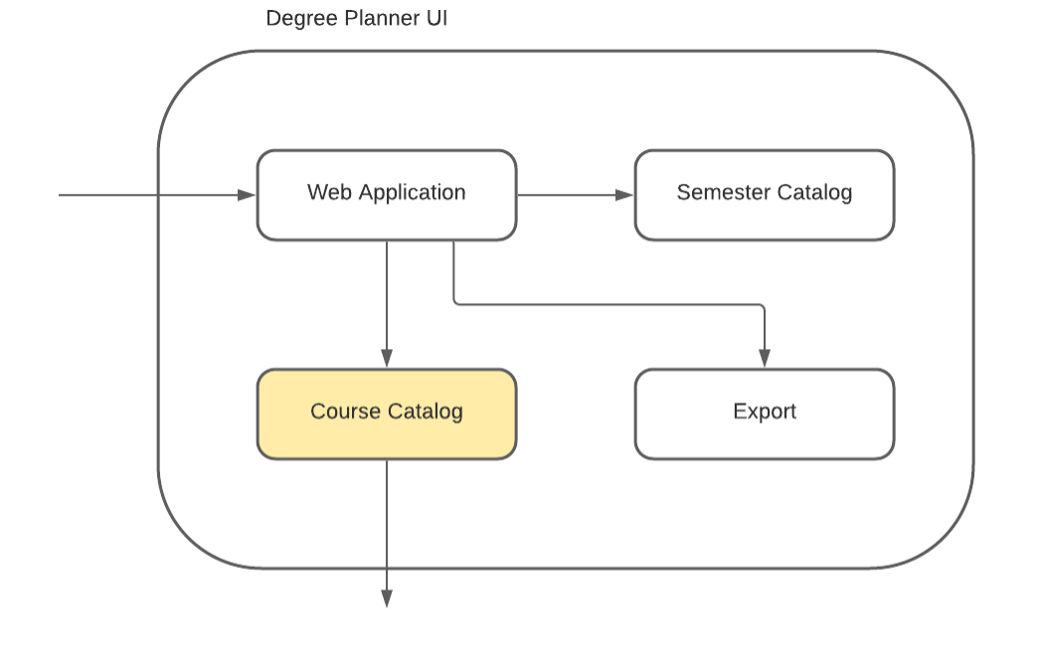
\includegraphics[width=0.60\textwidth]{images/CourseCatalog}
 \caption{Course Catalog subsystem}
\end{figure}

\subsubsection{Assumptions}
\begin{itemize}
\begin{item}
The user must have Internet connection.
\end{item}
\begin{item}
The subsystem gets the raw data from the Firebase layer.
\end{item}
\begin{item}
The subsystem fetches the up-to-date required data from the Firebase layer.
\end{item}
\begin{item}
The subsystem cannot modify data fetched from the Firebase database. It does not provide any functionality to modify data and no data changes should be made in this subsystem.
\end{item}
\end{itemize}

\subsubsection{Responsibilities}
This subsystem will take input, i.e., major, from the web application subsystem, and fetch the corresponding list of courses. Since the database only provides raw data, this subsystem will process each query to create a course object. The list of course objects will then pass to the Web application subsystem.

\subsubsection{Subsystem Interfaces}

\begin {table}[H]
\caption {Course Catalog subsystem interfaces} 
\begin{center}
    \begin{tabular}{ | p{1cm} | p{3cm} | p{2cm} | p{7cm} |}
    \hline
    ID & Description & Inputs & Outputs \\ \hline
    \#1 & Fetch data & \pbox{3cm}{Text} & \pbox{7cm}{Database response with the list of courses from selected major}  \\ \hline
    \#2 & Process data & \pbox{3cm}{Queries} & \pbox{7cm}{List of objects}  \\ \hline
    \end{tabular}
\end{center}
\end{table}

\subsection{Semester Catalog}
Semester catalog subsystem acts as the interface between the Degree Planner UI layer and Dashboard layer. It will read data, i.e., the starting semester, from the user information, and sends it to the Web application subsystem.

\begin{figure}[h!]
	\centering
 	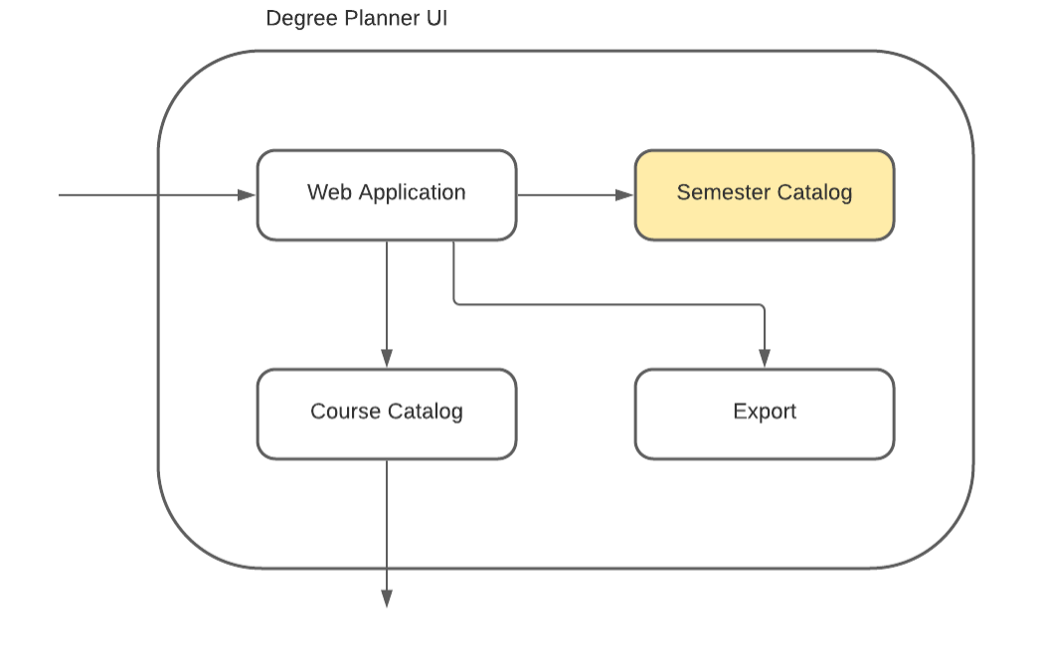
\includegraphics[width=0.60\textwidth]{images/SemesterCatalog}
 \caption{Semester Catalog subsystem}
\end{figure}

\subsubsection{Assumptions}
\begin{itemize}
\begin{item}
The user must have Internet connection.
\end{item}
\begin{item}
The subsystem cannot modify data fetched from the Dashboard. It does not provide any functionality to modify data and no data changes should be made in this subsystem.
\end{item}
\end{itemize}

\subsubsection{Responsibilities}
This subsystem automatically reads the user's starting semester and returns the list of all valid and available semesters to the Web application subsystem. That is, the estimated duration for pursuing a degree in the department of Computer Science and Engineering at the University of Texas at Arlington is 4 years; therefore, the maximum duration for degree completion would be 10 years. The list of semesters will include the starting semester and all subsequent semesters in the next 10 years.

\subsubsection{Subsystem Interfaces}

\begin {table}[H]
\caption {Semester Catalog subsystem interfaces} 
\begin{center}
    \begin{tabular}{ | p{1cm} | p{3cm} | p{2cm} | p{7cm} |}
    \hline
    ID & Description & Inputs & Outputs \\ \hline
    \#1 & Fetch data & \pbox{2cm}{N/A} & \pbox{7cm}{List of semesters in the next 10 years from the staring semester}  \\ \hline
    \end{tabular}
\end{center}
\end{table}

